\section{完备空间中的基本算子定理}
\label{sec:lop-fundamental-theorems}

前面几节的估计都要求直接找到一个常数，控制单位球上的全部输入。实际问题中我们手里常常只有较弱的信息：每个固定输入上的输出有界；方程对每个右端都有唯一解；或者输入、输出同时收敛时极限相容。

对矩阵，这些信息已经足够，因为矩阵只有有限多列，每一列都有界就够了。无穷多列时，统一的常数要靠完备性来保证。三个定理都建立在第~\ref{chap:metric-spaces}章的Baire纲定理之上：完备度量空间不能写成可数个无内点闭集之并。

每个结论都要分别核对三件事：定义域是否完备，取值空间是否完备，算子是否定义在整个空间上。我们还要区分几种“好”的性质：逐输入有界与统一有界，代数上可逆（存在逆映射）与稳定可逆（逆映射有界）。

\subsection{一致有界原理}
\label{sec:lop-uniform-boundedness}

第~\ref{chap:linear-functionals}章对连续线性泛函族证明了：每个固定向量上的观测有界，整族的范数就有统一上界。这里把同样的论证用于取值于一般赋范空间的算子族，所得结论称为\term{一致有界原理}（uniform boundedness principle）。

\begin{theorem}[一致有界原理]
\label{thm:lop-uniform-boundedness}
设$X$是Banach空间，$Y$是赋范空间，$\{T_\alpha\}_{\alpha\in\Lambda}\subseteq\mathcal B(X,Y)$。若对每个$x\in X$都有$\sup_\alpha\lVert T_\alpha x\rVert<\infty$，则
\begin{equation}
 \sup_{\alpha\in\Lambda}\lVert T_\alpha\rVert<\infty.
 \label{eq:lop-uniform-boundedness}
\end{equation}
\end{theorem}

\begin{proof}
对$n\geq1$令
\[
 F_n=\{x\in X:\lVert T_\alpha x\rVert\leq n\text{ 对一切}\alpha\text{ 成立}\}.
\]
每个集合$\{x:\lVert T_\alpha x\rVert\leq n\}$是连续函数$x\mapsto\lVert T_\alpha x\rVert$的下水平集，因而闭；$F_n$是它们的交，也是闭集。由假设，每个$x$属于某个$F_n$，所以$X=\bigcup_nF_n$。

$X$完备，由Baire纲定理，某个$F_n$有内点：存在$x_0$与$r>0$使闭球$\overline B(x_0,r)\subseteq F_n$。对$\lVert z\rVert\leq r$，$x_0+z$与$x_0$都属于$F_n$，于是对一切$\alpha$，
\[
 \lVert T_\alpha z\rVert\leq\lVert T_\alpha(x_0+z)\rVert+\lVert T_\alpha x_0\rVert\leq2n .
\]
按线性缩放，$\lVert T_\alpha\rVert\leq2n/r$对一切$\alpha$成立。
\end{proof}

三个条件各司其职。算子的有界性使$F_n$闭；定义域的完备性通过Baire纲定理在某一层中找到一个球；线性把这个球平移到原点并缩放到单位球。取值空间的完备性没有用到。

定义域不完备时结论可以失败。令$X$为只有有限个非零项的序列全体，配$\ell^2$范数，它不完备。令$T_nx=nx_n$（取值于$\mathbb F$）。对每个$x\in X$，当$n$大于$x$最后一个非零项的位置时$T_nx=0$，所以$\sup_n\lvert T_nx\rvert<\infty$。

但$\lvert T_ne_n\rvert=n$，所以$\lVert T_n\rVert=n$无界。逐输入有界本身不是统一有界，二者之间的桥梁正是完备性。

\paragraph{强收敛极限的有界性}
一致有界原理回答了第~\ref{sec:lop-operator-convergence}节留下的问题。设$X$是Banach空间，$T_n\in\mathcal B(X,Y)$，且对每个$x$，$T_nx$在$Y$中收敛，记极限为$Tx$。收敛序列有界，所以$\sup_n\lVert T_nx\rVert<\infty$对每个$x$成立，由定理得
\[
 K=\sup_n\lVert T_n\rVert<\infty.
\]
于是$T$线性，并且
\[
 \lVert Tx\rVert=\lim_n\lVert T_nx\rVert\leq K\lVert x\rVert,
\]
$T$是有界算子。强算子收敛不能保证统一误差趋于零，却至少保证了统一的范数上界与极限的有界性。

\subsection{开映射定理}
\label{sec:lop-open-mapping}

由输出恢复输入，要同时满足三个要求：给定的输出有原像（存在），原像只有一个（唯一），输出上的小误差只造成输入上的小误差（稳定）。方阵可逆就同时满足这三条；无限维中它们会分离。

第~\ref{chap:topological-spaces}章把开集的像仍为开集的映射称为开映射，这与连续性要求的“开集的原像为开集”方向相反。对线性算子，开映射性质恰好给出逆向的误差估计，这就是下面的\term{开映射定理}（open mapping theorem）。

\begin{theorem}[开映射定理]
\label{thm:lop-open-mapping}
设$X,Y$是Banach空间，$T\in\mathcal B(X,Y)$是满射。则存在$\delta>0$使
\begin{equation}
 B_Y(0,\delta)\subseteq T(B_X(0,1)),
 \label{eq:lop-open-mapping}
\end{equation}
从而$T$是开映射。特别地，每个$y\in Y$都有原像$x$满足$\lVert x\rVert\leq2\delta^{-1}\lVert y\rVert$。
\end{theorem}

定理说的是：满射不仅保证每个输出都有原像，还保证能选到一个范数受控的原像。证明分两步：先用Baire纲定理得到输出球落在输入球之像的闭包中，再用逐步修正残差去掉闭包。

\begin{proof}
记$B_r=B_X(0,r)$。第一步，像的闭包含有输出球。由满射，
\[
 Y=\bigcup_kT(B_k)=\bigcup_k\overline{T(B_k)}.
\]
$Y$完备，由Baire纲定理，某个$\overline{T(B_k)}$含有开球$B_Y(y_0,\rho)$。对$\lVert y\rVert<\rho$，$y_0+y$与$y_0$都在$\overline{T(B_k)}$中，二者之差属于$\overline{T(B_k)-T(B_k)}\subseteq\overline{T(B_{2k})}$。

所以$B_Y(0,\rho)\subseteq\overline{T(B_{2k})}$。令$\eta=\rho/(2k)$，按线性缩放得
\[
 B_Y(0,\eta/2^j)\subseteq\overline{T(B_{2^{-j}})}\qquad(j\geq0).
\]

第二步，逐步修正残差。任取$\lVert y\rVert<\eta$。由第一步，存在$x_1\in B_1$使$\lVert y-Tx_1\rVert<\eta/2$。残差$y-Tx_1$落在$B_Y(0,\eta/2)$中，于是存在$x_2\in B_{1/2}$使$\lVert y-Tx_1-Tx_2\rVert<\eta/4$。如此继续，得到$x_j$满足
\[
 \lVert x_j\rVert<2^{1-j},\qquad\Bigl\lVert y-T\sum_{i\leq j}x_i\Bigr\rVert<\eta/2^j .
\]

第三步，用输入空间的完备性求和。$\sum_j\lVert x_j\rVert<2$，部分和是$X$中的柯西列；$X$完备，所以$x=\sum_jx_j$存在且$\lVert x\rVert<2$。由$T$连续，$Tx=y$。这说明$B_Y(0,\eta)\subseteq T(B_2)$，取$\delta=\eta/2$即得式~\eqref{eq:lop-open-mapping}。

第四步，验证开映射。设$U\subseteq X$开，$x\in U$，取$\varepsilon>0$使$B_X(x,\varepsilon)\subseteq U$。则
\[
 T(U)\supseteq Tx+\varepsilon T(B_1)\supseteq B_Y(Tx,\varepsilon\delta),
\]
所以$T(U)$开。

最后证明原像的估计。设$y\neq0$，$y^\prime=\delta y/(2\lVert y\rVert)$落在$B_Y(0,\delta)$中，由式~\eqref{eq:lop-open-mapping}有$x^\prime\in B_1$使$Tx^\prime=y^\prime$。令$x=2\lVert y\rVert x^\prime/\delta$，则$Tx=y$且$\lVert x\rVert\leq2\delta^{-1}\lVert y\rVert$。
\end{proof}

第一步只得到闭包：闭包中的点只能被像逼近，未必是像。第二步把“可以逼近”变成“可以达到”，代价是输入球的半径从$1$放大到$2$，并且必须用到$X$的完备性。图~\ref{fig:lop-open-mapping}用一个二维线性映射画出这个修正过程。

\begin{BookInlineFigure}
  \centering
  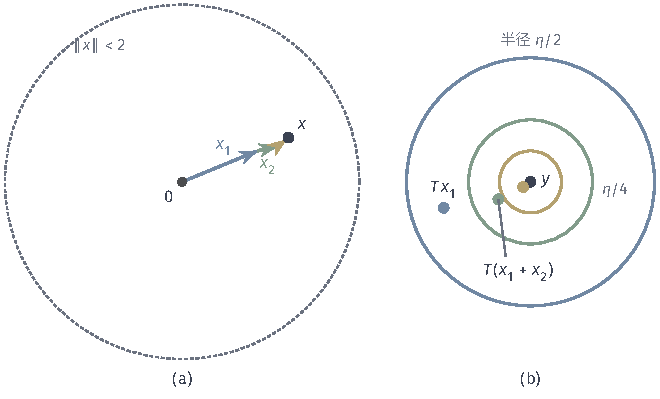
\includegraphics[width=111.725mm]{figures/04-spaces-measures-and-geometry/03-function-spaces/tikz/lop-open-mapping/figure.pdf}
  \caption{开映射定理证明中的残差修正，取$T=\operatorname{diag}(1,0.7)$，$\eta=1$作示意。(a)输入空间中修正量满足$\lVert x_j\rVert<2^{1-j}$，部分和收敛到原像$x$，$\lVert x\rVert<2$（虚线圆）。(b)输出空间中，近似$Tx_1$落在以$y$为心、半径$\eta/2$的圆内（蓝），加上修正后$T(x_1+x_2)$落入半径$\eta/4$的圆内（绿），第三次修正落入半径$\eta/8$的圆内（黄）。}
  \label{fig:lop-open-mapping}
\end{BookInlineFigure}

把开映射定理用于双射，原像的选取就是唯一的，于是逆映射自动连续。这一推论称为\term{有界逆定理}（bounded inverse theorem）。

\begin{theorem}[有界逆定理]
\label{thm:lop-bounded-inverse}
设$X,Y$是Banach空间，$T\in\mathcal B(X,Y)$是双射。则$T^{-1}\in\mathcal B(Y,X)$，并且
\begin{equation}
 \lVert T^{-1}\rVert\leq\delta^{-1},
 \label{eq:lop-bounded-inverse}
\end{equation}
其中$\delta$为开映射定理中的常数。
\end{theorem}

\begin{proof}
$T^{-1}$的线性来自$T$的线性。设$y\neq0$，$0<t<\delta$，由式~\eqref{eq:lop-open-mapping}，$ty/\lVert y\rVert$有原像落在$B_X(0,1)$中；$T$是单射，所以这个原像就是$T^{-1}(ty/\lVert y\rVert)$。于是
\[
 \lVert T^{-1}y\rVert<\frac{\lVert y\rVert}{t}.
\]
令$t\to\delta$，得$\lVert T^{-1}y\rVert\leq\delta^{-1}\lVert y\rVert$。
\end{proof}

\paragraph{代数可逆与稳定可逆}
有界逆定理说，在Banach空间之间，有界线性双射自动是稳定的：代数可逆就推出稳定可逆。条件不能省。$\ell^2$上的对角算子$A$是单射，它把$\ell^2$一一地映到像$\operatorname{Ran}A$上，在像上有逆映射$A^{-1}(y_n)=(ny_n)$。

这个逆相当于对角矩阵$\operatorname{diag}(1,2,3,\ldots)$，它无界：$\lVert A^{-1}e_n\rVert=n$，输出上$e_n/n$大小的误差会在恢复时变成长度为$1$的输入误差。原因在于$\operatorname{Ran}A$只是$\ell^2$中稠密而不闭的子空间（第~\ref{sec:lop-range-kernel}小节），按$\ell^2$范数不完备，定理的条件不成立。

开映射提供的正是局部误差估计：在原点附近半径$\delta$的输出球中，每个输出都有半径$1$以内的原像。线性把这一局部信息推广到所有尺度，就得到$\lVert T^{-1}y\rVert\leq\delta^{-1}\lVert y\rVert$。代数可逆只给出逆映射的存在；稳定可逆还要求这个统一的常数，二者在完备空间之间才自动重合。

\paragraph{两个完备范数的比较}
有界逆定理的一个直接用途是比较范数。设线性空间$X$在两个范数$\lVert\cdot\rVert_a$、$\lVert\cdot\rVert_b$下都完备，且$\lVert x\rVert_a\leq C\lVert x\rVert_b$。

恒等映射作为从$(X,\lVert\cdot\rVert_b)$到$(X,\lVert\cdot\rVert_a)$的映射是有界双射，其逆也有界，于是存在$C^\prime$使$\lVert x\rVert_b\leq C^\prime\lVert x\rVert_a$，两个范数等价。第~\ref{sec:lop-inclusions}节的$C[0,1]$上，$\lVert f\rVert_1\leq\lVert f\rVert_\infty$而两范数不等价，这与定理并不矛盾：$C[0,1]$在$\lVert\cdot\rVert_1$下不完备。

\subsection{闭图判别}
\label{sec:lop-closed-graph}

直接估计$\lVert Tx\rVert\leq C\lVert x\rVert$有时很困难。另一种思路是只检验一个较弱的条件：若输入$x_n\to x$，并且输出$Tx_n$也收敛到某个$y$，那么$y$是否必定等于$Tx$？这个条件不要求先证明输出收敛，只要求输入、输出同时收敛时极限相容。写成几何语言，就是算子的图
\begin{equation}
 \mathcal G(T)=\{(x,Tx):x\in D(T)\}\subseteq X\times Y
 \label{eq:lop-graph}
\end{equation}
在乘积范数$\lVert(x,y)\rVert=\lVert x\rVert+\lVert y\rVert$下是闭集。

$X,Y$都完备时，$X\times Y$也完备。下面的\term{闭图定理}（closed graph theorem）说明，对定义在整个完备空间上的算子，这个较弱的条件已经足够。

\begin{theorem}[闭图定理]
\label{thm:lop-closed-graph}
设$X,Y$是Banach空间，$T:X\to Y$是定义在整个$X$上的线性算子。则$T$有界当且仅当$\mathcal G(T)$在$X\times Y$中闭。
\end{theorem}

\begin{proof}
若$T$有界，$x_n\to x$推出$Tx_n\to Tx$，所以$Tx_n\to y$时$y=Tx$，图闭。

反过来，设图闭。它是Banach空间$X\times Y$的闭线性子空间，本身是Banach空间。第一坐标投影$\pi(x,Tx)=x$是从$\mathcal G(T)$到$X$的有界线性映射，因为$\lVert x\rVert\leq\lVert(x,Tx)\rVert$。它是双射，因为$T$定义在整个$X$上，每个$x$恰好对应图中一点。

由有界逆定理，$\pi^{-1}$有界：存在$C$使
\[
 \lVert x\rVert+\lVert Tx\rVert\leq C\lVert x\rVert,
\]
于是$\lVert Tx\rVert\leq C\lVert x\rVert$。
\end{proof}

图闭的条件同时考察输入与输出的极限：只知道$x_n\to x$而不知道$Tx_n$是否收敛，就无从检验；只看输出收敛而不管输入，也不能确定极限属于谁的图。定理的作用是把这个“两侧相容”的条件升级为有界性，代价是要求定义域为整个Banach空间。

\paragraph{处处有定义的对称算子有界}
设$T:H\to H$定义在整个Hilbert空间上，且$\langle v,Tx\rangle=\langle Tv,x\rangle$对一切$x,v$成立。若$x_n\to x$且$Tx_n\to w$，则对任意$v$，
\[
 \langle v,w\rangle=\lim_n\langle v,Tx_n\rangle=\lim_n\langle Tv,x_n\rangle=\langle Tv,x\rangle=\langle v,Tx\rangle ,
\]
所以$w=Tx$，图闭，$T$有界。这里没有估计任何范数，只用了对称性和内积的连续性。反过来说，无界的对称算子，例如适当定义域上的微分算子，不可能定义在整个Hilbert空间上。

\paragraph{定义域只是子空间时}
若$T$只定义在子空间$D(T)\subseteq X$上，图闭不再推出有界。回到求导$D:C^1[0,1]\subseteq C[0,1]\to C[0,1]$，两侧都用一致范数。它的图是闭的：若$f_n\to f$且$f_n^\prime\to g$都按一致范数，则在
\[
 f_n(x)=f_n(0)+\int_0^xf_n^\prime(t)\,\mathrm dt
\]
两边取极限，一致收敛允许在积分号下取极限，得到
\[
 f(x)=f(0)+\int_0^xg(t)\,\mathrm dt.
\]
所以$f\in C^1[0,1]$且$f^\prime=g$。

可是第~\ref{sec:lop-derivative-boundedness}小节已经用$\sin(2\pi nx)$说明$D$在一致范数下无界。两者不矛盾：$D(D)=C^1[0,1]$在一致范数下不完备，闭图定理的条件不满足。图闭的算子称为\term{闭算子}（closed operator）。

\paragraph{图范数}
对闭算子$T$，在定义域上换用\term{图范数}（graph norm）
\begin{equation}
 \lVert x\rVert_T=\lVert x\rVert_X+\lVert Tx\rVert_Y.
 \label{eq:lop-graph-norm}
\end{equation}
映射$x\mapsto(x,Tx)$把$(D(T),\lVert\cdot\rVert_T)$等距地映到图$\mathcal G(T)$上。当$X,Y$完备时，图作为闭子空间完备，所以$(D(T),\lVert\cdot\rVert_T)$是Banach空间，而$\lVert Tx\rVert_Y\leq\lVert x\rVert_T$说明$T$在新范数下有界。

对求导，图范数正是$\lVert f\rVert_{C^1}$。这就兑现了第~\ref{sec:lop-derivative-boundedness}小节的说法：配上$C^1$范数后定义域完备，同一个作用规则成为Banach空间之间的有界算子。

因此，把基本定理用于定义在真子空间上的算子之前，必须先确认所用的范数使定义域完备。第~\ref{chap:sobolev-spaces}章的Sobolev范数沿用同样的思想，用积分范数同时控制函数和它的弱导数。
